\chapter{Nodos}
	\label{chap:nodo_de_red}

El capitulo \ref{chap:nodo_de_red} describe la arquitectura de los miembros de la red propuesta. El contenido se aborda en el siguiente orden: En primer lugar se presenta el formato de paquete y el \textit{handshake} entre nodos para el intercambio de información. A continuación se describe la arquitectura del router  y su correspondiente interfaz de red para la interconexión con elementos de procesamiento. La siguiente sección presenta la arquitectura del nodo \textit{rebotador}, un elemento único de este trabajo. Finalmente se presenta un caso de estudio, donde un router es conectado a un núcleo de cifrado de algoritmo DES\cite{chapter0:NIST:1977:DES}. La figura \ref{fig:ch4_nodo} muestra un diagrama a alto nivel de los módulos que integran a un acelerador de hardware basado en NoC.
.
\begin{figure}
	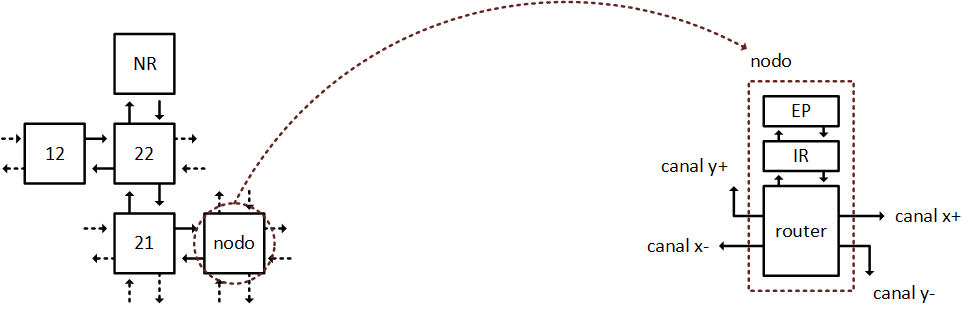
\includegraphics[width=\linewidth]{figures/ch4_nodo.png}
	\caption
		{	
			Cada nodo de red es una isla de procesamiento en el acelerador. Las líneas de interconexión entre nodos se denominan canales. EP: Elemento de procesamiento, IR: Interfaz de red y NR: Nodo Rebotador.
		}
	\label{fig:ch4_nodo}
\end{figure}

\section{Protocolo de comunicacion}
	\label{sec:protocolo_comunicacion}

El protocolo de comunicaciones esta formado por el formato de paquete y la secuencia de control entre routers. El formato de paquete determina el tamaño de la carga util de información a ser transmitida, ademas de establecer campos de control para el calculo de ruta de un paquete y su posterior procesamiento en el elemento funcional de un nodo.

La secuencia de control entre routers determina el intercambio de señales que indica a un nodo la llegada de un nuevo paquete a uno de sus puestos de entrada. Ademas de proporcionar el servicio anterior, la secuencia de control permite el envió/recepción de créditos entre routers para evitar la perdida de paquetes debido a la falta de espacio de almacenamiento temporal en un encaminador.










\subsection{Formato de paquete}
	\label{subsec:formato_de_paquete}

La infraestructura para el desarrollo de aceleradores de este trabajo implementa elementos de procesamiento homogéneos, con bloques de datos de trabajo de longitud fija para todos ellos. El uso de paquetes de datos de trabajo homogéneos simplifica loa mecanismos de control requeridos para la decodificación de estos, eliminando la necesidad de campos destinados al control de flujo de datagramas de longitud variable.

\begin{figure}
	\begin{center}
		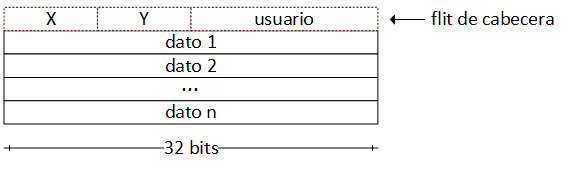
\includegraphics[scale=0.8]{figures/ch4_organizacion_paquete.png}
	\end{center}
	\caption
		{	
			No existe una restricción en el número de flits para el transporte de información dentro de un paquete, sin embargo, el incremento de estas unidades de transporte acarrea consigo una mayor congestión en la red además de un incremento en la cantidad de almacenamiento temporal requerido por cada uno de los puertos del encaminador. El flit de cabecera contiene la información necesaria para permitir que un paquete sea entregado a su destino.
		}
	\label{fig:ch4_organizacion_paquete}
\end{figure}

Todos los paquetes están formados por un flit de cabecera seguido de cualquier número de flits para el transporte de datos. El número de flits que conforman un paquete está determinado por la aplicación, y debe de especificarse de manera previa a la síntesis del acelerador. El tamaño de paquete definido en tiempo pre-síntesis hace innecesario la inclusión de un flit de final de paquete.

El contenido de los flit de datos es transparente para los nodos del sistema, los routers e interfaces de red no tienen mecanismos para la discriminación de campos o formatos dentro de ellos. El flit de cabecera es un caso particular, en el, el número y longitud de campos es fijo y tienen un profundo impacto en el funcionamiento de la lógica de los routers. La figura \ref{fig:ch4_flit_cabecera} muestra la distribución de campos a lo largo de un flit de cabecera.

\begin{figure}
	\begin{center}
		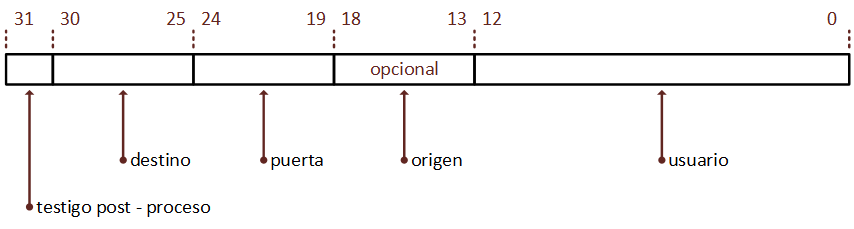
\includegraphics[scale=0.7]{figures/ch4_flit_cabecera.png}
	\end{center}
	\caption
		{	
			Formato de flit de cabecera. El uso del campo \textit{origen} permite la implementación de algoritmos de encaminamiento basados en el modelo \textit{odd-even}. En caso de omitir el uso del campo origen durante el proceso de planificación de ruta, su espacio puede anexarse al campo \textit{usuario} para ampliar su longitud.
		}
	\label{fig:ch4_flit_cabecera}
\end{figure}

Una vez que un paquete a sido aceptado por un elemento de procesamiento, el campo \textit{testigo post-proceso} es activado para indicar que el paquete está en busca de una puerta de salida de la red, y no requiere competir por el uso de un elemento de procesamiento. Los campos \textit{destino}, \textit{puerta} y \textit{origen} almacenan una dirección de nodo formada por una dupla \{\textit{x,y}\}. Estos campos tienen una longitud fija de 6 bits. La distribución de bits de los campos para la representación de direcciones puede variar dependiendo de la geometría de la red, por ejemplo, se puede asignar un mayor número de bits a la dimensión \textit{x} en caso que se desee una geometría rectangular en lugar de una cuadrada. El uso de 6 bits como espacio de direcciones permite tener en la red un máximo de 64 nodos. Es posible extender el espacio de direccionamiento sacrificando capacidad de almacenamiento de los campos \textit{usuario} y \textit{origen} para extender de manera efectiva las direcciones que pueden representarse por medio de los campos destino y puerta.

El campo \textit{usuario} ofrece la posibilidad de implementar mecanismos de \textit{Calidad de Servicio (QoS)}. Un ejemplo del uso de este campo es la verificación de recepción de todos los paquetes liberados a la red para su procesamiento. En el escenario anterior, el campo usuario es utilizado para incluir un identificador a cada paquete, mediante este número se puede corroborar que todos los paquetes liberados para procesamiento en la red han sido recibidos en en la puerta de salida correcta. Los servicios \textit{QoS} pueden implementarse directamente en hardware o software dependiendo de la interfaz para la extracción de datos del acelerador.










\subsection{Protocolo de enlace}
	\label{subsec:protocolo_de_enlace}

El protocolo de enlace entre dos routers asegura la interpretación correcta de una solicitud de envió de paquete, así como la coordinación entre ambos elementos para evitar la perdida de datos debido a una insuficiencia de espacio de almacenamiento en el nodo destino.

El \textit{handshake} entre dos routers se lleva a cabo mediante 4 señales de control:

\begin{itemize}[noitemsep]
	\item par\_disp - Señal par diferencial positivo (origen). 
	\item par\_disn - Señal par diferencial negativo (origen).
	\item rec\_crt  - Señal de retorno de créditos (origen).
	\item env\_crt  - Señal de retorno de créditos (destino).
\end{itemize}


El protocolo implementa un par de señales diferenciales dedicadas para el control de transferencia de paquetes, un cambio de estado en el par diferencial indica al router receptor la llegada de un nuevo tren de flits. El uso de un par diferencial dedicado en lugar de un campo de identificación en el flit de cabecera reduce la posibilidad de la creación de paquetes espurios resultado de la corrupción de datos. El sistema de señalización permite la integración de servicios como transferencias tipo \textit{broadcast} o servicios QoS. La figura \ref{fig:ch4_w_protocolo_comunicacion} muestra la transmisión de dos paquetes entre encaminadores.


\begin{figure}
	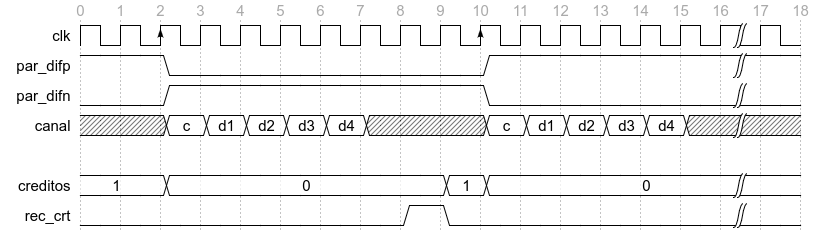
\includegraphics[width=\linewidth]{figures/ch4_w_protocolo_comunicacion.png}
	\caption
		{	
			El protocolo de comunicación involucra un intercambio de señales (\textit{handshake}) de dos pasos. La transmisión inicia con la inversión de la señales del par diferencial (ciclo 2), el intercambio finaliza con la aserción de la señal rec\_crt la cual indica que el router destino tiene espacio disponible para la recepción de un paquete adicional.
		}
	\label{fig:ch4_w_protocolo_comunicacion}
\end{figure}


El protocolo se encuentra fuertemente ligado al control de enlace basado en créditos\footnote{Capitulo \ref{ch:topicos_selectos} sección - Control a nivel de enlace basado en créditos}, ya que la transmisión de paquetes se ve detenida cuando el router destino ha agotado todos sus espacios de almacenamiento temporal como se muestra en el ciclo 2 de la figura \ref{fig:ch4_w_protocolo_comunicacion}. Durante el flanco positivo del octavo ciclo de operación, el router destino libera un espacio de almacenamiento y envia un crédito al router origen mediante la señal de paso de crédito (rec\_crt). Un ciclo de trabajo es necesario para que el router origen procese la recepción del crédito y reinicie el envió de paquetes como se muestra en la figura \ref{fig:ch4_w_protocolo_comunicacion} durante el décimo ciclo. El protocolo de comunicación no implementa un medio de corrección de errores de transmisión en la capa física o de enlace del encaminador, esta tarea se delega a capas superiores para mantener un nivel bajo de complejidad en los routers de la red.










\section{Arquitectura del router}
	\label{sec:arquitectura_router}

El router esta diseñado para operar bajo el esquema de conmutación de paquetes utilizando la técnica \textit{virtual cut-through}, el control de flujo se basada en el uso de \textit{créditos}. El diseño permite definir de manera previa a la síntesis el ancho de canales de entrada/salida y la capacidad de almacenamiento temporal(\textit{buffers}) para la retención de paquetes. El router puede ser utilizado para formar redes con topología torus o malla.  

De manera interna el modulo está organizado en dos particiones lógicas, una dedicada al transporte de datos (\textit{camino de datos}) y una segunda partición para el control de la dirección en la que la información fluye a través del módulo (\textit{camino de control}). La tabla \ref{tab:unidades_arq} muestra las principales unidades de la arquitectura.


% Please add the following required packages to your document preamble:
% \usepackage{booktabs}
% \usepackage[table,xcdraw]{xcolor}
% If you use beamer only pass "xcolor=table" option, i.e. \documentclass[xcolor=table]{beamer}
\begin{table}[]
\centering
\begin{tabular}{@{}p{0.1\linewidth}p{0.1\linewidth}p{0.8\linewidth}lll@{}}
\toprule
\rowcolor[HTML]{9B9B9B} 
{\color[HTML]{FFFFFF} \begin{tabular}[c]{@{}l@{}}Plano\\ lógico\end{tabular}} & {\color[HTML]{FFFFFF} Unidad}                                                     & {\color[HTML]{FFFFFF} Descripción}                                                                                                                                                                                                                                                                                                    \\ \midrule
\rowcolor[HTML]{EFEFEF} 
Datos                                                                         & \begin{tabular}[c]{@{}l@{}}Puerto de\\ entrada\end{tabular}                       & Unidad de recepción de paquetes. De manera interna se encarga de el manejo del protocolo de comunicación así como del almacenamiento temporal de paquetes en transito. Este modulo tiene comunicación directa con unidad de generación de peticiones para disparar el proceso de solicitud de recursos para la salida de información. \\
Datos                                                                         & Crossbar                                                                          & Lógica para la interconexión de entradas y salidas del router.                                                                                                                                                                                                                                                                        \\
\rowcolor[HTML]{EFEFEF} 
Datos                                                                         & \begin{tabular}[c]{@{}l@{}}Puerto de\\ salida\end{tabular}                        & Unidad de manejo de protocolo de comunicación así como de recepción de créditos desde routers vecinos.                                                                                                                                                                                                                                \\
Control                                                                       & \begin{tabular}[c]{@{}l@{}}Unidad de\\ generación\\ de \\ peticiones\end{tabular} & Modulo encargado del calculo de puertos de salida productivos para la propagación de un paquete. Ademas del calculo de ruta, este modulo se encarga de mantener la solicitud de recursos activa hasta que un arbitro otorgue recursos a su petición.                                                                                   \\
\rowcolor[HTML]{EFEFEF} 
Control                                                                       & \begin{tabular}[c]{@{}l@{}}Segmento de\\ control de\\ crossbar\end{tabular}       & Lógica de control para la configuración del crossbar.                                                                                                                                                                                                                                                                                 \\ \bottomrule
\end{tabular}
\caption{Unidades principales del encaminador.}
\label{tab:unidades_arq}
\end{table}

Es importante definir los términos \textit{canal} y \textit{puerto}, ya que se utilizan para la descripción del encaminador. El término \textit{canal} se utiliza para referirse al medio físico que enlaza dos routers vecinos. El término \textit{puerto} está asociado a los modulo que se encargan de la recepción y decodificación de los paquetes entrantes a un router.

Internamente el router presenta una estructura uniforme, donde cada canal entrante al modulo esta conectado a un puerto de entrada que se encarga de la recepción de paquetes, los puertos de entrada proporcionan los campos de dirección a una unidad generadora de peticiones la cual solicita el uso de un puerto de salida para cada paquete en transito. La administración de puertos de salida se lleva a cabo de manera distribuida, donde existe un segmento de control de crossbar encargado de recibir peticiones para el uso de un puerto de salida especifico, arbitrar entre todas las peticiones activas y seleccionar una de ellas para otorgar un enlace entre el puerto de entrada solicitante y el puerto de salida solicitado. La conexión entre ambos puertos se lleva a cabo mediante el crossbar del router. La figura \ref{fig:ch4_slice_arq} muestra un segmento perteneciente a la interconexión entre un puerto de entrada, el crossbar y un puerto de salida, este arreglo se replica para cada uno de los canales de entrada/salida del encaminador.

\begin{figure}
	\begin{center}
		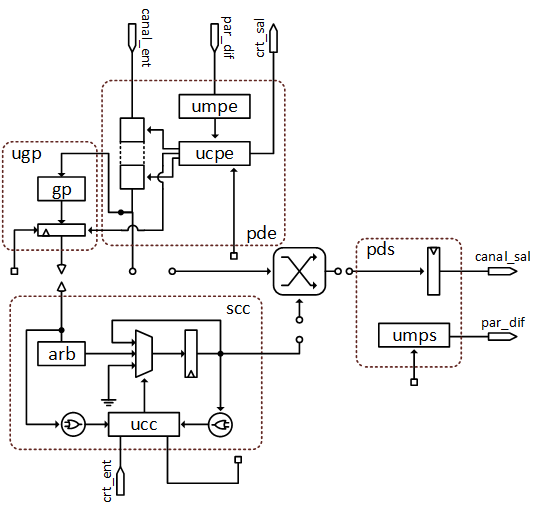
\includegraphics[scale=0.7]{figures/ch4_slice_arq.png}
	\end{center}
	\caption
		{	
			Diagrama general de un segmento de los caminos de control y datos entre un puerto de salida y uno de entrada. Glosario: UMPE - Unidad de Manejo de Protocolo de Entrada. UCPE - Unidad de Control de Puerto de Entrada. UCC - Unidad de Control de Crossbar. UMPS - Unidad de Manejo de Protocolo de Salida. SCC - Segmento de Control de Crossbar. UGP - Unidad de Generación de Peticiones. PDE - Puerto de Entrada. PDS - Puerto de Salida. 
		}
	\label{fig:ch4_slice_arq}
\end{figure}

El plano de control del router está formada por módulos \textit{UMPE} - Unidad de Manejo de Protocolo de entrada, \textit{UMPS} (Unidad de Manejo de Protocolo de Salida) y \textit{SCC} (Segmento de Control de Crossbar). Los módulos \textit{UMPE} (Unidad de Manejo de Protocolo de Entrada) y \textit{UMPS} (Unidad de Manejo de Protocolo de Salida) se encargan del cumplimiento de la señalización a través de pares diferenciales requerida por el protocolo de comunicación, el UMPE detecta el cambio en el par diferencial, almacena el nuevo estado de las lineas y genera un habilitador para iniciar el proceso de recepción de un paquete. Por su parte el modulo UMPS recibe una habilitador para generar un cambio valido en el par diferencial para indicar a un router vecino que se a iniciado la transmisión de un tren de flits. Gran parte de la responsabilidad de de las dos unidades mencionadas anteriormente es el mantener el correcto orden de la transiciones en el par diferencial, un desfase en el patrón de cambios derivara en una incorrecta interpretación de paquetes entrantes.

La unidad SCC integra un arbitro y a un modulo de retención de resultado de arbitraje controlado por la unidad \textit{UCC} (Unidad de Control de Crossbar). Las unidades SCC se encargar de administrar un puerto de salida de manera exclusiva por lo que existe una de estas unidades por cada conexión a un vecino del router. El arbitro de la unidad SCC recibe las peticiones generadas desde los módulos UGP, como resultado del proceso de arbitraje una de las peticiones es aceptada y se procede a configurar el crossbar para crear un enlace desde el puerto de entrada ganador y el puerto de salida custodiado por la SCC. La unidad UCC se encarga de retener la configuración del crossbar el tiempo necesario para permitir el paso de todo los flits pertenecientes a un paquete. Adicionalmente, la unidad UCC integra el manejo de creditos para el puerto de salida al cual se encuentra administrando.

A Partir de esta sección se utilizará de manera indiferente los términos \textit{cola} o \textit{buffer} para referirse a la estructura de almacenamiento temporal ligado a los puertos de entrada. De igual forma, los términos \textit{estructura de interconexión} y \textit{crossbar} se utilizan de manera indistinta para hacer referencia a la malla de interconexión entre puertos de entrada y salida del router.










\subsection{Etapas de segmentación}
	\label{etapas_segmentacion}

El camino critico a través del router se encuentra segmentado por dos etapas registros. De manera adicional, los canales de entrada y salida se encuentran registrados, fungiendo como dos etapas adicionales de segmentación. La figura \ref{fig:ch4_segmentacion_entrada_salida} presenta las etapas de segmentación del router y las unidades que pertenecen a cada una de ellas.


\begin{itemize}[noitemsep]
	\item Almacenamiento de Flit (AF) - Esta etapa se activa con la recepción de un nuevo paquete. La unidad UMPE actualiza el estado del par diferencial de entrada y emite un testigo a la unidad UCPE para que inicie el proceso de recepción de un nuevo paquete. La unidad UCPE habilita al buffer del puerto para la captura de los flits entrantes.
	\item  Calculo de Ruta (CR)- Durante la recepción de un flit de cabecera la unidad GP calcula los puertos de salida que abonan a la entrega del paquete a su destino, ademas, genera las peticiones pertinentes. LA unidad GP mantienen el vector de peticiones a todos los puertos de salida relevantes para el paquete en transito. Una vez recibido un arbitraje favorable, esta unidad limpia el vector de peticiones actual y procede a atender peticiones de calculo de ruta pendientes en el buffer.
	\item Configuración de Crossbar (CC) - El vector de peticiones desde la unidad GP llega a los árbitros de cada puerto de salida, en caso de existir una petición, el arbitro determina el puerto de entrada que tendrá acceso al puerto de salida durante la ronda de arbitraje actual. La unidad UCC recibe el resultado del proceso de arbitraje y configura el crossbar de manera que el buffer del puerto de entrada ganador tenga un camino al puerto de salida requerido. La unidad UCC da aviso al puerto de entrada que su solicitud a sido aceptada y que el enlace con el puerto de salida se encuentra listo para la liberación del paquete.
	\item Paso de Crossbar (PC) - Una vez configurado el crossbar, los flits son transferidos uno a uno desde el buffer de entrada al registro del puerto de salida. Durante esta etapa de segmentación la unidad UCPE se encuentra activa habilitando el proceso de lectura de datos en el buffer de entrada.
\end{itemize}


\begin{figure}
	\begin{center}
		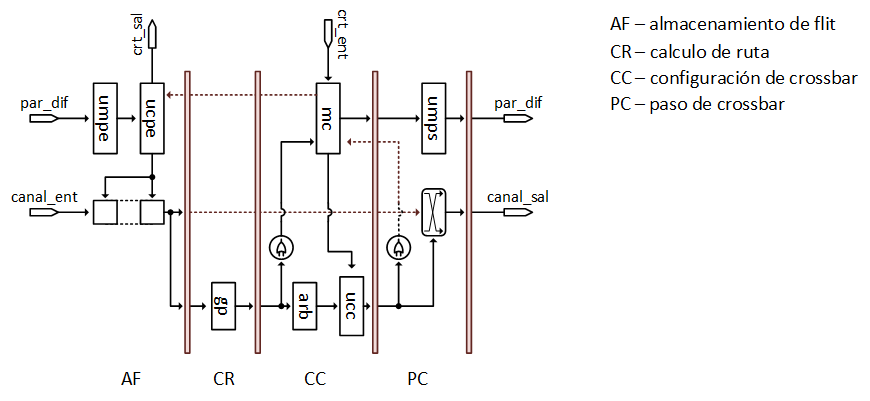
\includegraphics[width=\linewidth]{figures/ch4_segmentacion_entrada_salida.png}
	\end{center}
	\caption
		{	
			El buffer dentro de un  puerto de entrada funge como registro para el flit en transito durante el ciclo de reloj actual.
		}
	\label{fig:ch4_segmentacion_entrada_salida}
\end{figure}

El paso de un flit a través del encaminador toma 4 ciclos de reloj. A partir del dato previo es posible determinar el tiempo de viaje redondo de un crédito entre encaminadores vecinos como se muestra a continuación:

\begin{equation}
	\Delta_{cdt} =  \Delta_{we} + \Delta_{pe} + \Delta_{wd} + \Delta_{seg}  + \Delta_{ws}
	\label{eq:rtt}
\end{equation}

Donde $\Delta_{we}$ es el retador de propagación de crédito entre routers, $\Delta_{pe}$ es el tiempo de procesamiento requerido para asimilar un crédito entrante, $\Delta_{wd}$ representa el retardo de propagación del primer flit en dirección del siguiente salto, $\Delta_{seg}$ es la latencia para el paso de un flit a través de un router y $\Delta_{ws}$ es el retardo de propagación de un crédito retornando al router origen. La figura \ref{fig:ch4_rtt} muestra la secuencia de la ecuación \ref{eq:rtt}. Un $\Delta_{cdt} = 8$ ciclos de reloj requiere de al menos $2F$ espacios de almacenamiento\footnote{Consultar capitulo \ref{ch:topicos_selectos} para mas detalles en el calculo de capacidad de buffer.} para mantener el máximo desempeño de manera constante entre conmutadores vecinos. 

\begin{figure}
	\begin{center}
		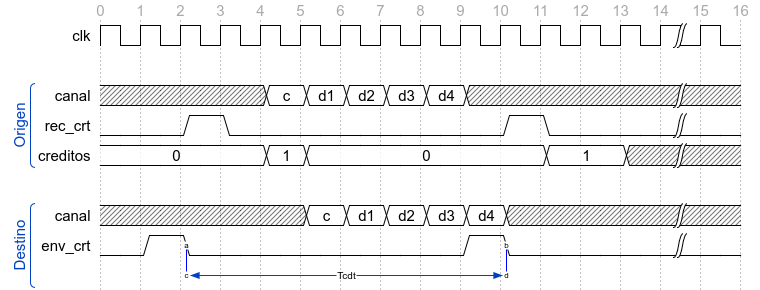
\includegraphics[width=\linewidth]{figures/ch4_w_rtt.png}
	\end{center}
	\caption
		{	
			Forma de onda del intercambio de un paquete entre dos routers. Se requiere de 8 ciclos de reloj para que un crédito realice un viaje redondo entre los dos routers.
		}
	\label{fig:ch4_rtt}
\end{figure}










\subsection{Puerto de entrada}
	\label{puerto_entrada}

El puerto de entrada (figura \ref{fig:ch4_puerto_entrada}) extiende su operación durante dos etapas de segmentación del router. Durante la etapa AF, la unidad UMPE detecta el cambio en el par diferencial, a partir de este evento se generan dos acciones, por una parte la unidad actualiza su banco de estado interno mientras se genera una señal para la unidad UCPE que a su vez iniciara con la captura de flits he indicara que es necesario iniciar el proceso de solicitud de recursos a las unidades SCC. Durante la etapa CR la unidad GP obtiene un vector de peticiones resultante del calculo de ruta para el paquete en transito, al final de esta etapa el vector se registra y se propagan las peticiones a las unidades SCC correspondientes

\begin{figure}
	\begin{center}
		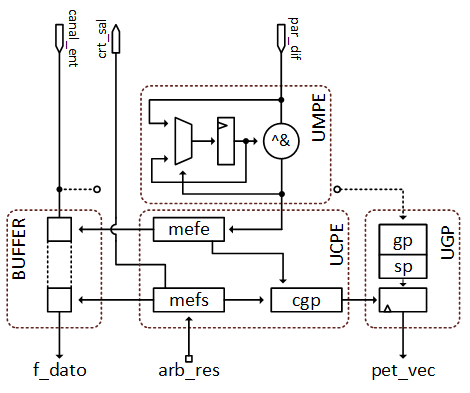
\includegraphics[scale=0.8]{figures/ch4_puerto_entrada.png}
	\end{center}
	\caption
		{	
			Todos los puertos de entrada del router son estructuras homogéneas, de manera que el IP es reutilizable y presenta el mismo comportamiento sin importar al canal que se encuentre asignado.
		}
	\label{fig:ch4_puerto_entrada}
\end{figure}

La unidad UCPE esta formada internamente por dos maquinas de estado finito: MEFE (Maquina de Estado Finito de Entrada) y MEFS (Maquina de Estado de Salida). MEFE genera las señales de control de escritura para el buffer, y en conjunto con la unidad CGP (Control de Generación de Peticiones), determina el origen de los campos de dirección para el calculo de ruta y si el resultado de de este ultimo proceso debe ser propagado a las unidades SCC. La figura \ref{fig:ch4_pde_fsm} a) muestra el modelado de la maquina de estados MEFE.

La unidad CGP lleva un registro interno del numero de paquetes almacenados en el buffer del puerto, ademas de conocer estado de las unidades MEFE y MEFS. A partir de los datos anteriores, la unidad indica a la UGP (Unidad Generadora de Peticiones) si debe iniciar un nuevo proceso de generación de peticiones. La tabla \ref{tab:CGP} presenta el árbol de decisiones de la unidad CGP.

La maquinada de estado finito MEFS ejerce control sobre las tareas de lectura de datos en el buffer así como el  retorno de créditos al router vecino inmediato. La maquina de estados esta modelada por el diagrama que se muestra en el apartado b) de la figura \ref{fig:ch4_pde_fsm}. Es importante notar que el regreso de un crédito se puede llevar a cabo al momento de la recepción de una resolución favorable por parte del arbitro de cualquier unidad SCC, inclusive si se encuentra en medio de la captura de un paquete entrante. La liberación del crédito no corre el riesgo de un desbordamiento en el buffer de entrada como resultado del uso de la técnica Virtual Cut Through, donde el espacio para la recepción de un paquete esta asegurado en el siguiente router, en otras palabras una vez que la transmisión de un paquete ha iniciado se tiene la certeza que todos los flits pertenecientes al mismo serán desalojados del buffer del puerto de entrada, habilitando el espacio para la recepción de un paquete mas.


% Please add the following required packages to your document preamble:
% \usepackage{booktabs}
% \usepackage[table,xcdraw]{xcolor}
% If you use beamer only pass "xcolor=table" option, i.e. \documentclass[xcolor=table]{beamer}
\begin{table}[]
\centering
\begin{adjustbox}{width=1\textwidth}
\begin{tabular}{@{}cccccc@{}}
\toprule
\rowcolor[HTML]{343434} 
{\color[HTML]{FFFFFF} MEFE actual} & {\color[HTML]{FFFFFF} MEFE siguiente} & {\color[HTML]{FFFFFF} MEFS actual} & {\color[HTML]{FFFFFF} MEFS siguiente} & {\color[HTML]{FFFFFF} Paquetes en buffer} & {\color[HTML]{FFFFFF} habilitador UGP} \\ \midrule
NEW                                & PUSH                                  & IDLE                               & IDLE                                  & 0                                         & Activo                                 \\
\rowcolor[HTML]{EFEFEF} 
X                                  & X                                     & ACK                                & PULL                                  & \textgreater0                             & Activo                                 \\
X                                  & X                                     & PULL                               & PULL                                  & \textgreater0                             & Activo                                 \\
\rowcolor[HTML]{EFEFEF} 
X                                  & X                                     & X                                  & X                                     & X                                         & Inactivo                               \\ \bottomrule
\end{tabular}
\end{adjustbox}
\caption{Solo los estados definidos como 'activo' dispararan la propagación de peticiones a las unidades SCC del router. Los casos no definidos en la tabla mantienen deshabilitado el registro de la unidad CGP.}
\label{tab:CGP}
\end{table}


\begin{figure}
	\begin{center}
		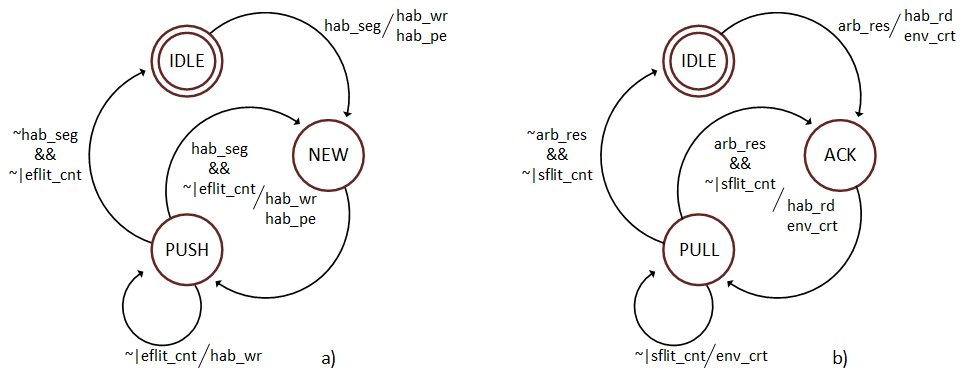
\includegraphics[width=\linewidth]{figures/ch4_pde_fsm.png}
	\end{center}
	\caption
		{	
			a) Maquina de estados finitos de entrada (MEFE). b) Maquina de estados finitos de salida (MEFS).
		}
	\label{fig:ch4_pde_fsm}
\end{figure}

Dentro  de la unidad UGP se lleva el proceso de calculo de ruta, este ultimo ofrece como resultado un vector de peticiones para los puertos de salida que resultan productivos para el avance del paquete en transito. El algoritmo \textit{West-First minimal} ofrece múltiples rutas al ser un algoritmo parcialmente adaptativo. La generación de peticiones simultaneas puede acarear inconsistencias en la operación de un router, por ejemplo: dos unidades SCC reciben una petición de una unidad UGP, ambas unidades SCC aceptan la petición y crean un enlace entre el puerto de entrada y sus correspondientes puertos de salida, como resultado el paquete en el buffer es transmitido a través de los puertos de salida asignados, creando un duplicado del paquete. La unida UGP puede agregar módulos para el manejo de casos particulares como el anteriormente descrito, en el escenario anterior un modulo SP (Selector de Peticiones) se encarga de seleccionar solo una petición del vector generado en base a un esquema de prioridad fija y el estado de las unidades SCC del router.

El router descrito en este trabajo implementa un modulo SP, el cual trabaja aplicando un proceso de filtrado de dos etapas. Durante la primera etapa se reciben todas las peticiones generadas por el modulo GP, solo las peticiones a unidades SCC que se encuentren disponibles en este momento son enviadas a la segunda etapa de filtrado. La segunda etapa consiste en la aplicación de un esquema de prioridad fijo que implementa el siguiente orden:

\begin{enumerate*}
\item Elemento de procesamiento
\item Puerto 'X+'
\item Puerto 'Y+'
\item Puerto 'X-'
\item Puerto 'Y-'
\end{enumerate*}










\subsection{Crossbar}
	\label{Crossbar}

\begin{figure}
	\begin{center}
		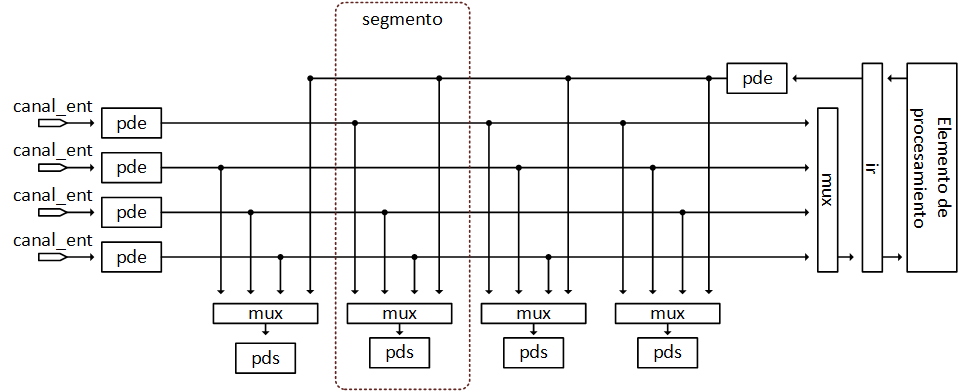
\includegraphics[scale=0.7]{figures/ch4_crossbar.png}
	\end{center}
	\caption
		{	
			Cada unidad SCC genera el vector de control para cada uno de los segmentos del crossbar. Los segmentos están configurados para mantener sus lineas de salida en cero mientras no se encuentren paquetes en transito, la inclusión de una un valor constante no repercute en el numero de entradas al multiplexor, solo en la señales de control del mismo.
		}
	\label{fig:ch4_crossbar}
\end{figure}

El medio de interconexión entre puertos está implementado mediante una estructura tipo \textit{crossbar}, la cual  consiste en una cascada de multiplexores independientes para la conexión de varios puertos de entrada con un puerto de salida. Los algoritmos de encaminamiento WFM (West Firts Minimal) y DOR XY (Dimensional Order Routing XY) no permiten el reenvió de un paquete en la misma dirección por la cual ingreso al router,  por lo que cada segmento del crossbar no requiere proporcionar un servicio completo de interconexión. Dado que $\delta$  tiene un valor de 4 para los router tipo malla, y se cuenta con un canal de salida para el elemento de procesamiento de un nodo, cada segmento del crossbar requiere de un multiplexor de 4 entradas y una salida. Un multiplexor es implementado en un dispositivo reconfigurable mediante el uso de LUTs (Look Up tables),  en la mayoria de los casos dichos elementos cuentan con un 6 entradas y dos salidas, permitiendo la implementación de multiplexores en combinaciones de 4x1 o 2x2. La restricción en la implementación de multiplexores requiere que cada segmento del croosbar sea sintetizado como una estructura tipo cascada en lugar de una jerarquía plana con un solo nivel. La figura \ref{fig:ch4_crossbar} muestra un diagrama a bloques de la infraestructura de interconexión interna del router. 










\subsection{Segmento de Control de Crossbar}
	\label{scc}

\begin{figure}
	\begin{center}
		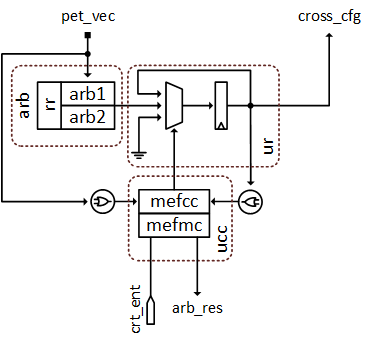
\includegraphics[scale=0.9]{figures/ch4_unidad_scc.png}
	\end{center}
	\caption
		{	
			Las unidades SCC son responsables de mantener el control del numero de créditos disponibles  en el router vecino inmediato, por lo cual reciben de manera directa la señal de recepción de créditos. El tiempo de proceso de un crédito es igual a un ciclo de reloj debido al cambio de estado de la maquina de estados finito que se encarga de administrar el proceso. La señal 'pet\_vec' representa el vector formado por todas las peticiones enviadas a la unidad SCC desde los puertos de entrada ligados a ella.
		}
	\label{fig:ch4_unidad_scc}
\end{figure}

Cada unidad SCC se encarga de el arbitraje y retención de enlaces entre un puerto de entrada y uno de salida. Internamente se encuentra formado por un par de árbitros en cascada (ARB1 Y ARB2) y un generador de prioridad Round Robin (RR), una Unidad de Retención (UR), una unidad de control de corssbar (UCC) formada por dos maquinas de estado finito: MEFCC (Maquina de Estado Finito de Control de Crossbar) y MEFMC (Maquina de Estado Finito para Manejo de Créditos).

El esquema convencional de un arbitro de prioridad variable se muestra en la figura \ref{fig:ch4_arbitro} a). Este modelo de arbitro no es funcional dentro de dispositivos reconfigurables debido a la meta estabilidad en la señal de acarreo que forma una relación cíclica a lo largo del arbitro. Para superar la restricción del ciclo combinacional, se implemento el diseño de arbitro en cascada de la figura \ref{fig:ch4_arbitro} b). En este, se duplica el hardware para iniciar una cadena de acarreo que supone un estado bajo a su entrada, la salida de acarreo del primer arbitro es utilizada por el segundo arbitro del sistema en cascada.  Si el valor de acarreo de salida para el primer arbitro del arreglo es 0, ambos árbitros coincidirán en la resolución del proceso de arbitraje, en caso contrario, el resultado del segundo arbitro producirá la salida correcta del proceso de arbitraje. El vector de prioridad $P_{x}$ es generado por medio del algoritmo Round-Robin.

\begin{figure}
	\begin{center}
		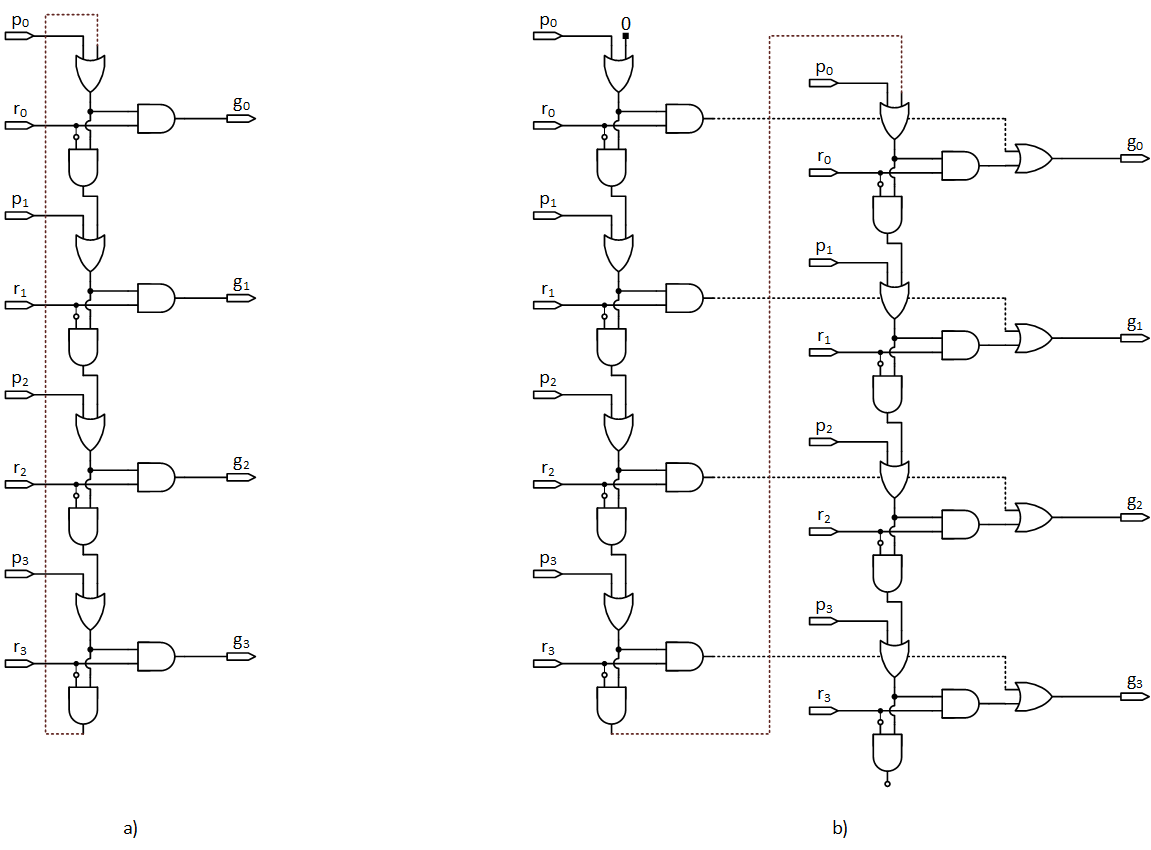
\includegraphics[width=\linewidth]{figures/ch4_arbitro.png}
	\end{center}
	\caption
		{	
			a) Implementación tradicional de arbitro con sistema de prioridad dinámica. b) Implementación de arbitro para dispositivos reconfigurables. La eliminación del ciclo combinacional en la cadena de acarreo del arbitro es necesario para su porte a dispositivos FPGA.
		}
	\label{fig:ch4_arbitro}
\end{figure}

La salida del arbitro es un vector utilizando codificación 'binario natural' para representar el puerto de entrada al cual se le ha otorgado la concesión del uso del puerto de salida. El uso de binario natural reduce el numero de bits necesarios para representar el resultado del proceso de arbitraje, ademas permite utilizar el vector directamente para la configuración de los multiplexores que conforman un segmento del crossbar.

La unidad UCC en conjunto con el modulo UR administra el vector de configuración que se inyectara al crossbar. El modulo UR permite seleccionar entre el registro del vector generado por el arbitro, retener la configuración actual o enviar la señal cross\_cfg a estado bajo. La decisión anterior recae en la unidad MEFCC, la cual decide si un nuevo proceso de arbitraje es necesario tomando en cuenta los siguientes parámetros: solicitudes existentes desde puertos de entrada (pet\_pen) y disponibilidad de créditos (crd\_disp). La MEFCC inicia un proceso de arbitraje siempre que el puerto de salida se encuentre en reposo, se cuente con créditos disponibles y exista una petición activa. Una vez obtenido el resultado de la unidad ARB, este permanecerá almacenado en el registro de la unidad UR durante el tiempo necesario para la transferencia de los flits de un paquete desde el buffer hasta el puerto de salida. En caso de no existir peticiones activas, la unidad MEFCC mantiene el vector de configuración para el crossbar en estado bajo.

El manejo de créditos se lleva a cabo mediante una maquina de estados en la unidad MEFMC, la cual responde a dos eventos: al momento del inicio de la transferencia de un paquete en dirección al router vecino, la unidad MEFMC disminuye el registro de créditos disponibles en una unidad, ya que el buffer del siguiente encaminador se encuentra almacenando el paquete enviado. Al recibir la liberación de un crédito por parte del siguiente encaminador, la unidad MEFMC incrementa el registro de créditos. Vale la pena mencionar que la liberación de créditos no se lleva  a cabo en la unida MEFMC, es tarea de la unidad MEFS la liberación de un crédito al router anterior como respuesta al inicio de un proceso de arbitraje en la unidad SCC. La figura \ref{fig:ch4_fsm_scc} presenta el modelado de ambas maquinas de estados de las unidades MEFCC y MEFMC.


\begin{figure}
	\begin{center}
		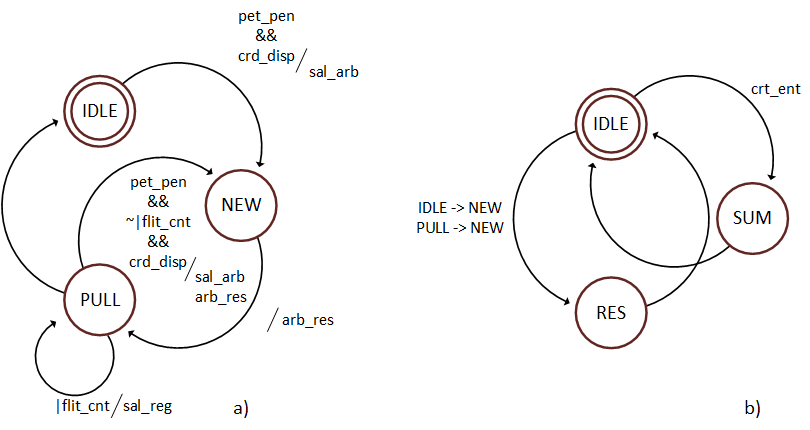
\includegraphics[scale=0.7]{figures/ch4_fsm_scc.png}
	\end{center}
	\caption
		{	
			a) Maquina de estado finito de la unidad MEFCC. b) Maquina de estado finito para la unidad MEFMC.
		}
	\label{fig:ch4_fsm_scc}
\end{figure}









\subsection{Puerto de Salida}
	\label{Puerto_salida}

El puerto de salida consta de un registro para almacenar de manera temporal un flit en transito al siguiente encaminador y un modulo UMPS. Este ultimo modulo opera de manera similar al modulo UMPE del puerto de entrada, su tarea es llevar registro del par diferencial el puerto de entrada y llevar a cabo el cambio de estado cuando se inicie la transmisión de un paquete.








\section{Arquitectura de Interfaz de Red}
	\label{sec:arq_ir}

Los paquetes de información en tránsito a través de la red utilizan el formato descrito en la sección \ref{subsec:formato_de_paquete}. El formato fue diseñado en orden de simplificar el hardware necesario para la decodificación y transporte de información tomando en cuenta las restricciones físicas que impone el ancho de canal entre routers. La información contenida en el paquete debe ser pre-procesada antes de ser inyectada a un elemento funcional de un nodo, y de igual forma el resultado entregado por una unidad funcional debe de ser encapsulado junto con los campos de control para formar un paquete.

La tarea de empaquetado/desempaquetado de información se lleva a cabo en las interfaces de red de cada nodo. La figura \ref{fig:ch4_interfaz_de_red_top} muestra el diagrama a bloques general de una interfaz de red. El encaminador del nodo interactúa con la interfaz de red como si se tratase de un encaminador vecino. La transferencia de información entre la interfaz de red y el encaminador se basa en el intercambio de paquetes y la entrega/recepción de créditos para mantener el control sobre el flujo de información.


\begin{figure}
	\begin{center}
		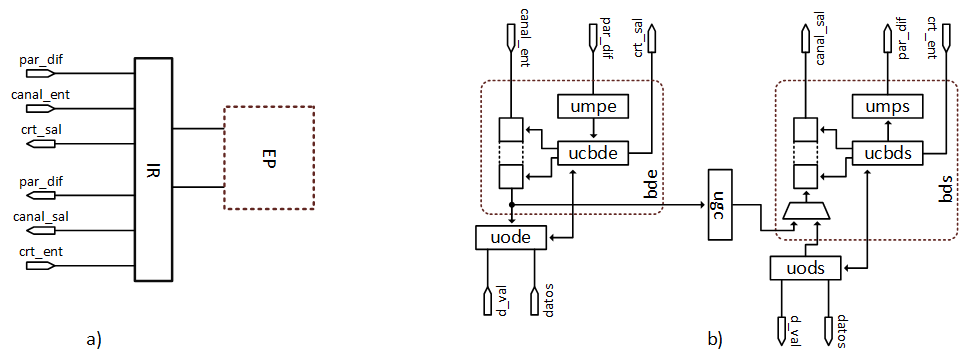
\includegraphics[width=\linewidth]{figures/ch4_interfaz_de_red_top.png}
	\end{center}
	\caption
		{	
			Interfaz de red. a) la interfaz de red se conecta al encaminador como un vecino más de la red. b) Las unidades UCBDE y UCBDS son versiones modificadas de la unidad UCPE del puerto de entrada.
		}
	\label{fig:ch4_interfaz_de_red_top}
\end{figure}


El elemento de procesamiento define las señales de control y datos involucrados en la interacción con la interfaz de red. El área de intercambio entre interfaz y elemento de procesamiento representa un desafío para la versatilidad de la red, ya que diferentes elementos de procesamiento requerirán interfaces de red a medida. Para facilitar la tarea de diseño de interfaces se ha dividido internamente el módulo en un bloque de entrada (BDE) y un bloque de salida (BDS) como se muestra en la figura \ref{fig:ch4_interfaz_de_red_top} \textit{b)}.

La áreas de interacción con el encaminador no requieren un análisis profundo ya que utilizan la misma filosofía de envío/recepción de paquetes entre routers, y de hecho, reutilizan los mecanismo de manejo de paquetes utilizados por los módulos UMPE, UMPS, MEFE y  MEFS de los puertos de entrada y unidades SCC del router.

EL bloque de entrada de la interfaz provee los datos de trabajo para el elemento de procesamiento, además de al menos una señal de control para indicar que los datos a la entrada del elemento de procesamiento son válidos y puede iniciar la captura del dato. Es trabajo del bloque de entrada es el reorganizar los flits de datos de un paquete de manera que se presenten en el formato nativo de trabajo del elemento de procesamiento, además de cumplir con cualquier protocolo de transferencia de información impuesto por este último.

Por su parte, el bloque de salida espera la finalización del trabajo llevado a cabo por el elemento de procesamiento. Una señal de control o una transacción de un protocolo de comunicación (\textit{handshake}) indica al bloque de salida que los datos son válidos y puede iniciar la captura de resultados. Los datos transmitidos por el elemento de procesamiento pueden encontrarse en tamaños de palabra diferentes a los de un flit, por lo que es tarea del bloque de salida reorganizar la información de manera que puedan empaquetarse previo a su liberación a la red.

El flit de cabecera no se envía al elemento de procesamiento, todo el trabajo de re-codificación de la información de la cabecera se lleva a cabo dentro de la interfaz de red en la Unidad de Generación de Cabecera (UGC). De manera ordinaria, el tratamiento que se le da a un flit de cabecera consiste en asignar el estado alto a su campo \textit{testigo post-proceso} y el intercambio de los campos \textit{destino} y \textit{puerta}. Los cambios al flit de cabecera ocasionan que el paquete viajando con los resultados no compita nuevamente por el uso de un elemento de procesamiento en ningún otro nodo de la red, además, su nueva dirección destino es una de las puertas de salida de la red.

Las unidades UCBDE y UCBDS son versiones modificadas de la unidad UCPE del puerto de entrada. Estas unidad agrega una señal gatillo para indicar que los datos en el buffer son validos o para indicar que los datos provenientes del elemento de procesamiento se encuentran listos para su transmisión a la red. Las unidades UODE (Unidad de Ordenamiento de Datos de Entrada) y UODS (Unidad de Ordenamiento de Datos de Salida) son unidades a medida para cada elemento de procesamiento que se conecte a un nodo de red.







\section{Caso de Estudio: encriptador DES}
	\label{sec:caso_des}

En esta sección se presenta el desarrollo de una interfaz de red para un bloque encriptador basado en el algoritmo DES \cite{chapter0:NIST:1977:DES}. El encriptador trabaja con dos bloques de 64 bits de longitud, uno de ellos contiene el conjunto de datos a encriptar, mientras el segundo bloque acarrea la llave de cifrado. El estándar de encriptación DES especifica el uso de claves de longitud de 56 bits, sin embargo, es una práctica común el agregar 1 bit de paridad por cada 7 bits que conforma la clave. El bit de paridad sirve para verificar la integridad de la clave de encriptación.
El elemento de encriptación recibe la frase original y la clave de cifrado en forma de una carga paralela como se muestra en la figura \ref{fig:ch4_interfaz_des}. La señal \textit{d\_val} se utiliza para indicar al encriptador que los datos en sus puertos de entrada son válidos y puede iniciar con su tarea.

Como resultado, el módulo DES regresa una palabra de 64 bits conteniendo la información cifrada. Se utiliza una segunda señal \textit{d\_val} para indicar a la interfaz de red que los datos en el puerto de salida del encriptador son válidos para su captura. Para complementar el control de flujo de información entre la interfaz de red y el encriptador se agrega la señal de control \textit{proc}, que funge como indicador de un retorno de crédito desde el núcleo DES. Cada vez que el núcleo de encriptación libera el resultado de su procesamiento al modulo UODS, un nuevo paquete desde el bloque BDE pasa al modulo UODE, la señal proc deja saber al bloque BDE que puede recibir un nuevo paquete desde la red ya que el dato almacenado en la unidad UODE ha sido consumido. 


\begin{figure}
	\begin{center}
		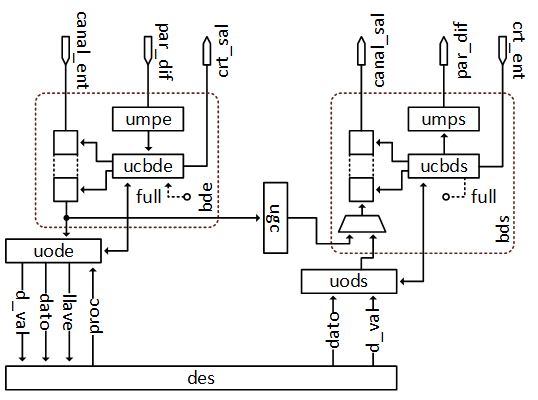
\includegraphics[scale = 0.8]{figures/ch4_interfaz_des.png}
	\end{center}
	\caption
		{	
			Las líneas de comunicación entre interfaz y elemento de procesamiento están definidas para acoplarse al formato utilizado por el elemento funcional. En este ejemplo se favorece una interfaz con de carga paralela de datos.
		}
	\label{fig:ch4_interfaz_des}
\end{figure}

Más a detalle, la unidad UODE está compuesta por un banco de registros y una unidad de control. El encriptador requiere que se alimente con los datos de trabajo de forma paralela, por lo tanto, cada registro del banco tiene un puerto de salida dedicado. El bus de datos de entrada del encriptador consta de dos palabras de 64 bits, por lo cual, suponiendo flits de 32 bits, se deduce que cada paquete de la red debe de estar formado por un flit de cabecera y 4 flits de datos.

El trabajo de la unidad UODE, mostrado en la figura \ref{fig:ch4_bloque_entrada_des}, inicia con el disparo de la señal \textit{d\_val}, esta dispara el ciclo de captura de flits desde el modulo bde. El tamaño del paquete (5 flits) se a especificado de manera previa a la síntesis del acelerador, por lo que la unidad de control (UC) esta programada de antemano para capturar el número de flits del paquete, el flit de cabecera no es procesado por el núcleo DES por lo que el modulo BDE no lo almacena. Con la captura de todos los flits de datos de un paquete, la unidad de control propaga la señal \textit{d\_val} para indicar al encriptador que un conjunto de datos esta disponible para ser consumidos en una nueva ronda de cifrado.


\begin{figure}
	\begin{center}
		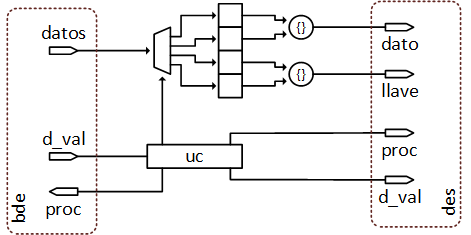
\includegraphics[scale=0.9]{figures/ch4_bloque_entrada_des.png}
	\end{center}
	\caption
		{	
			Las líneas de comunicación entre interfaz y elemento de procesamiento están definidas para acoplarse al formato utilizado por el elemento funcional. En este ejemplo se favorece una interfaz con carga de datos paralela.
		}
	\label{fig:ch4_bloque_entrada_des}
\end{figure}

La aserción de la señal proc por parte del núcleo indica que los datos disponibles en los puertos de salida a han sido consumidos, la unidad de control retransmite la señal proc al modulo BDE para indicar que un nuevo paquete de flits de datos puede ser enviado al modulo UODE. El envió de un nuevo paquete puede ser inhibido por la unidad BDS, en este escenario el bloque de salida tiene paquetes en cola esperando a ser transmitidos a la red, por lo que su buffer no cuenta con capacidad para la recepción de un nuevo resultado por parte del núcleo. La aserción de la señal \textit{full} inhibe la transmisión de un nuevo paquete a la unidad UODE.

El bloque de salida de la interfaz de red está formado por un par de registros para contener el resultado del proceso de cifrado. La unidad de control espera la confirmación por parte del núcleo del final de la ronda actual, una vez recibida la señal d\_val la unidad UODS captura el dato y retransmite la señal d\_val a la unidad BDS. La unidad DBS indica el inicio de la transmisión de datos por medio de la señal d\_acp. La espera a la confirmación por parte de la unidad BDS es necesaria ya que se requiere el ordenamiento del paquete en el buffer de transmisión, la unidad BDS inserta la cabecera proporcionada por la unidad UGC y posteriormente solicita el envió del dato recién capturado a la unidad UODS. El diagrama de la Unidad de Ordenamiento de Salida se presenta en la figura \ref{fig:ch4_bloque_salida_des}. La unidad UODS proporciona dos flit, haciendo un total de 3 flits contando con la cabecera del paquete, los flits restantes son generados con una carga útil vacía pero son necesarios para mantener el tamaño fijo de paquete de 5 flits.

\begin{figure}
	\begin{center}
		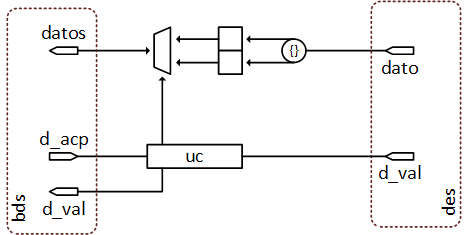
\includegraphics[scale=0.9]{figures/ch4_bloque_salida_des.png}
	\end{center}
	\caption
		{	
			Unidad UODS.
		}
	\label{fig:ch4_bloque_salida_des}
\end{figure}

 
